\documentclass[a4paper, 14pt]{extarticle}

\usepackage{../mystyle}

\begin{document}
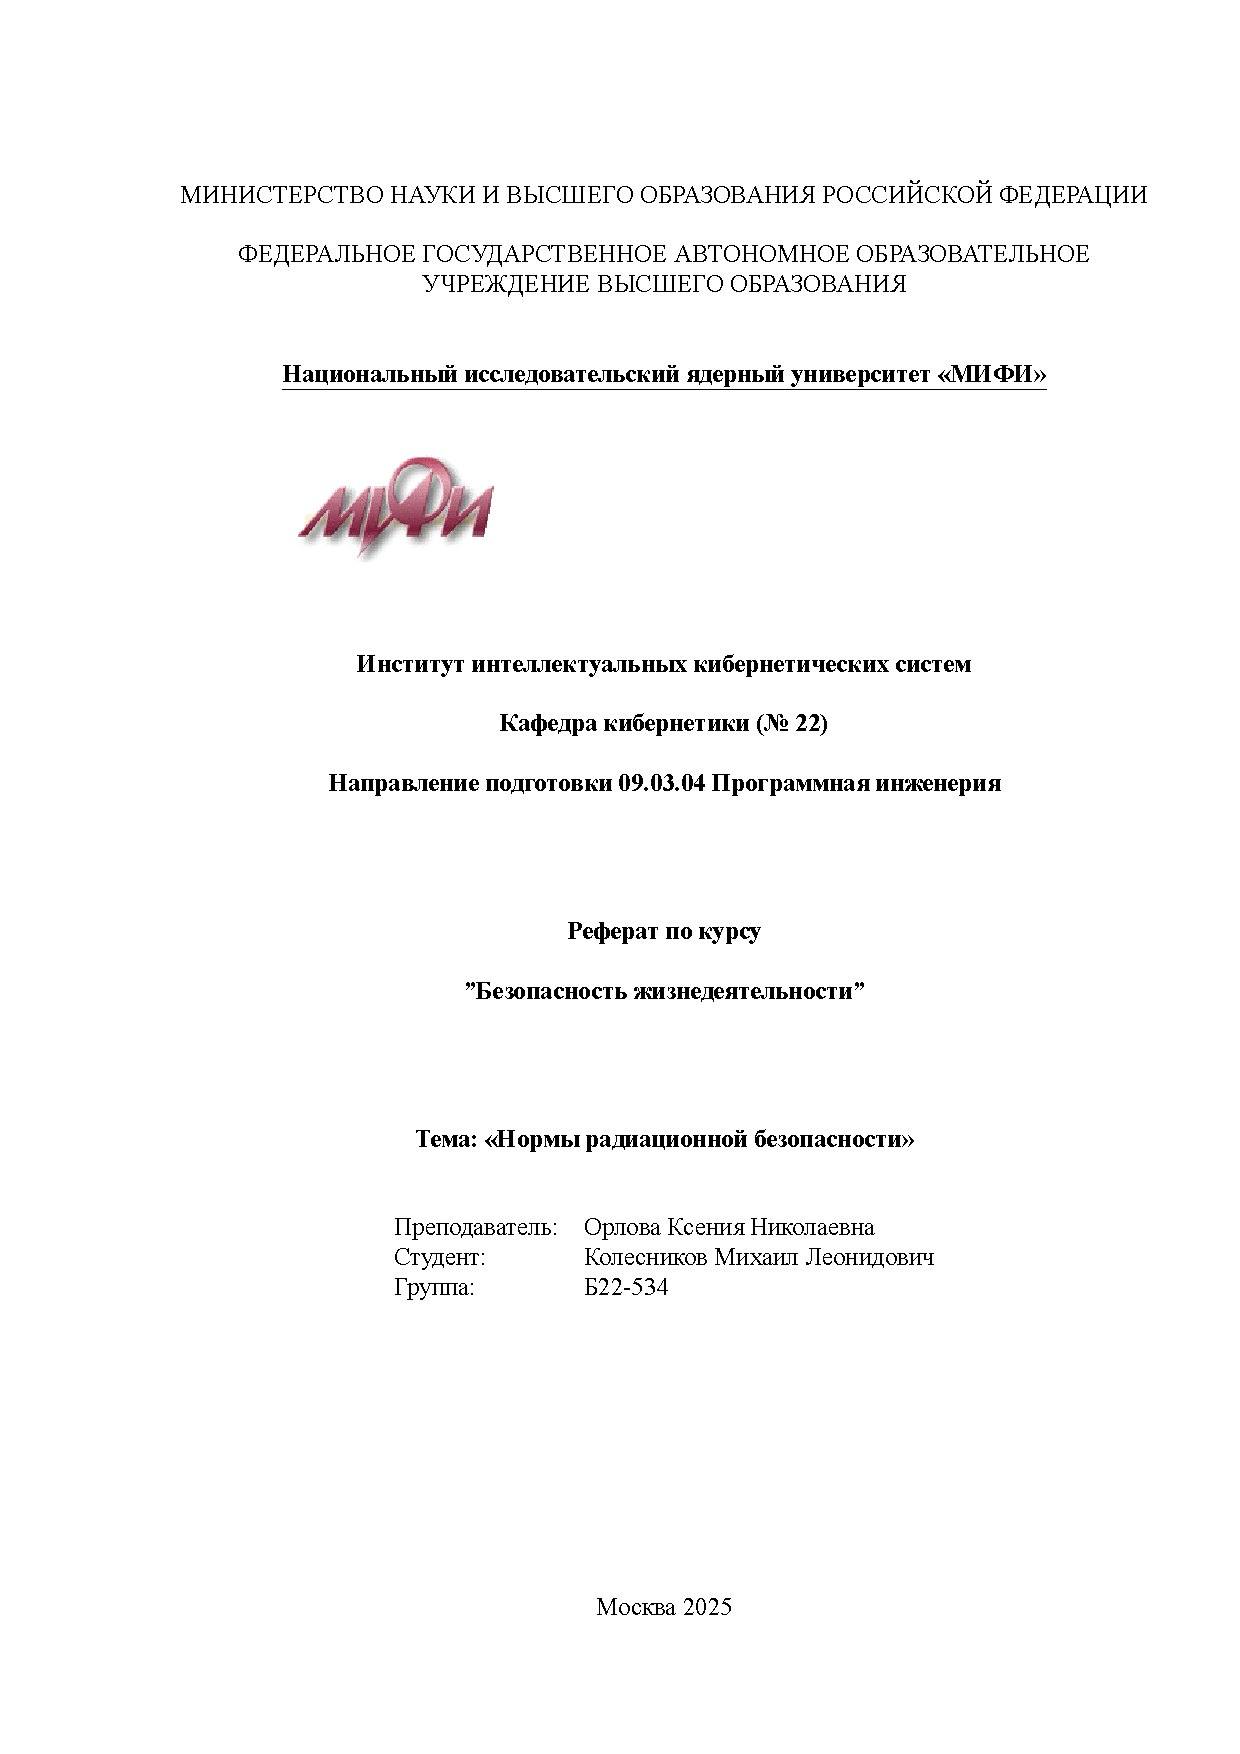
\includepdf[pages={1}]{../titul/titul.pdf}
\tableofcontents

\newpage

\section{Введение}

Радиационная безопасность остается одной из наиболее актуальных и стратегически важных проблем современности. С развитием атомной энергетики, медицины и промышленного применения радиоактивных материалов вопросы обеспечения безопасности жизнедеятельности приобретают критическое значение. Случаи радиационных инцидентов в прошлом, такие как аварии на Чернобыльской АЭС и Фукусима, продемонстрировали необходимость строгого регулирования использования радиоактивных веществ и обеспечения защиты населения, работников и окружающей среды.

Актуальность темы обусловлена многими факторами:

\begin{itemize}
    \item \textbf{Расширение применения радиационных технологий.} От диагностики и лечения заболеваний до промышленных процессов и энергетики — радиационные технологии находят применение в различных секторах, что требует универсальных и строгих норм безопасности.

    \item \textbf{Глобализация и международная интеграция.} Разные страны и международные организации разрабатывают собственные стандарты, что создает необходимость их анализа, сравнения и возможной гармонизации.

    \item \textbf{Эволюция научных исследований.} Новейшие исследования в области радиационной защиты, мониторинга и количественной оценки дозовых воздействий позволяют совершенствовать нормативы с целью минимизации возможного ущерба.
\end{itemize}

Цель данной работы — провести глубокий аналитический обзор нормативов радиационной безопасности, изучить противоречия между различными международными и национальными стандартами, критически оценить их практическое применение в различных отраслях, а также выявить тенденции в развитии нормативно-правового регулирования в данной области.

\section{Основная часть}

\subsection{Виды облучения}
\subsubsection*{По источникам излучения}

\begin{itemize}
    \item Внешнее облучение — от наружных источников излучения (космические лучи, воздействие природных или искусственных излучателей).
    \item Внутреннее — от радиоактивных веществ, попадающих внутрь организма человека с вдыхаемым воздухом, продуктами питания, с водой.
\end{itemize}

\subsubsection*{По времени действия излучения на объект}

\begin{itemize}
    \item Острое облучение — облучение, длительность которого не превышает нескольких часов, чаще всего составляя минуты.
    \item Пролонгированное облучение (протрагированное) — облучение, продолжающееся в течение многих дней, месяцев и лет.
    \item Хроническое облучение — длительное при низкой мощности дозы.
\end{itemize}

\subsubsection*{По зоне поражения}

\begin{itemize}
    \item Крупнопольное (широкопольное) облучение — облучение злокачественных новообразований, например лимфогранулематоза, большими полями в расчете на одновременное поражение основного очага и диссиминатов опухолевых клеток в регионарные лимфатические узлы.
    \item Локальное облучение (местное) — облучение отдельных участков (сегментов) тела.
    \item Общее (тотальное) облучение — облучение всего тела.
\end{itemize}

\subsection{Критериальные параметры норм радиационной безопасности}

ПД (предельные дозы) — это основные пределы доз облучения, которые не должны превышаться для различных категорий облучаемых лиц (например, персонала и населения). Они задают максимально допустимый уровень эффективной дозы, выражаемый в миллизивертах (мЗв) в год, например, 20 мЗв для персонала и 1 мЗв для населения. ПД являются ключевым критерием радиационной безопасности и служат ориентиром для установления других норм.

ПГП (предел годового поступления) — это допустимый уровень поступления конкретного радионуклида в организм человека за год, при котором ожидаемая доза облучения не превышает соответствующего предела годовой дозы (ПД). ПГП выражается в беккерелях (Бк) и применяется для оценки внутреннего облучения при монофакторном воздействии одного радионуклида через дыхание или пищу.

ДОА (допустимые среднегодовые объемные активности) — это нормативы, ограничивающие среднегодовую концентрацию радионуклидов в воздухе рабочей зоны или окружающей среды, при которых облучение не превышает ПД. ДОА связаны с ПГП, но применяются для контроля внешних условий и воздушной среды.

\subsection{Современные международные стандарты радиационной безопасности}

\begin{itemize}
    \item \textbf{Международная комиссия по радиационной защите (МКРЗ, ICRP)} --- независимая неправительственная организация, основанная в 1928 году, которая разрабатывает основные принципы и рекомендации по радиационной защите. Рекомендации МКРЗ являются фундаментом для международных норм и национальных стандартов многих стран.
    \item \textbf{Международное агентство по атомной энергии (МАГАТЭ)} --- разрабатывает и публикует нормы безопасности, основанные на рекомендациях МКРЗ и совместно с другими международными организациями (ВОЗ, МОТ, ФАО, АЯЭ/ОЭСР и др.). Нормы МАГАТЭ охватывают все этапы жизненного цикла источников излучения и направлены на минимизацию риска для здоровья и окружающей среды.
    \item Международные нормы безопасности представляют собой результат многолетних усилий по согласованию и гармонизации правил радиационной защиты на глобальном уровне. Они учитывают современный уровень научных знаний и опыта в области радиационной безопасности.
\end{itemize}

\subsubsection*{Основные принципы радиационной безопасности}

\begin{itemize}
    \item \textbf{Принцип обоснования}: любое использование источников ионизирующего излучения должно иметь оправданную пользу, превышающую потенциальный вред.
    \item \textbf{Принцип оптимизации}: уровни облучения должны быть максимально снижены с учётом разумных возможностей (ALARA --- \textit{As Low As Reasonably Achievable}).
    \item \textbf{Принцип нормирования}: установление предельных дозовых значений для различных категорий облучаемых (профессиональное облучение, население и др.).
\end{itemize}

\subsubsection*{Дозовые лимиты}

\begin{itemize}
    \item Для профессионального персонала (группа А) годовая эффективная доза не должна превышать 20 мЗв в среднем за любые 5 последовательных лет, но не более 50 мЗв в год.
    \item Для населения годовая эффективная доза не должна превышать 1 мЗв в среднем за любые 5 лет, но не более 5 мЗв в год.
    \item За весь период трудовой деятельности (50 лет) для персонала лимит составляет 1000 мЗв, а для населения за всю жизнь (70 лет) --- 70 мЗв.
\end{itemize}

\subsubsection*{Регулирование и применение}

\begin{itemize}
    \item Международные нормы служат основой для национального законодательства и стандартов радиационной безопасности в разных странах.
    \item В России, например, действуют нормы НРБ-99/2009, которые основаны на международных рекомендациях и регулируют допустимые уровни облучения и требования к безопасности.
    \item Международные нормы применяются на всех этапах использования радиационных источников --- от проектирования и эксплуатации до утилизации и ликвидации аварийных ситуаций.
\end{itemize}

\subsection{Российские нормативы: НПБ-99/2009 и ОСПОРБ-99/2010}

Нормы радиационной безопасности (НРБ) --- это санитарные нормы и правила, регулирующие допустимые уровни воздействия ионизирующего излучения на человека с целью защиты его здоровья при нормальных и аварийных условиях. В России действуют нормы НРБ-99/2009, введённые с 1 сентября 2009 года, которые устанавливают основные пределы доз облучения и требования по ограничению радиационного воздействия.

\begin{itemize}
    \item \textbf{Годовые пределы эффективной дозы облучения:}
          \begin{itemize}
              \item Для персонала, работающего с источниками ионизирующего излучения (группа А), --- 20 мЗв в среднем за любые последовательные 5 лет, но не более 50 мЗв в год.
              \item Для населения --- 1 мЗв в среднем за любые последовательные 5 лет, но не более 5 мЗв в год.
          \end{itemize}
          Эти дозы не включают облучение от естественных природных источников, медицинских процедур и радиационных аварий, для которых установлены отдельные ограничения.

    \item \textbf{Область применения норм:}
          \begin{itemize}
              \item Нормы распространяются на техногенные источники излучения при нормальной эксплуатации и в аварийных ситуациях, природные и медицинские источники.
              \item Исключены из регулирования космическое излучение на поверхности Земли и внутреннее облучение человека от природного калия-40, поскольку на них невозможно влиять.
          \end{itemize}

    \item \textbf{Дополнительные требования:}
          \begin{itemize}
              \item Контроль и ограничение доз облучения персонала с помощью индивидуальных дозиметров.
              \item Ограничение облучения от природных источников в производственных условиях --- эффективная доза не должна превышать 5 мЗв в год.
          \end{itemize}

    \item \textbf{Регулирующие документы:}
          \begin{itemize}
              \item НРБ-99/2009 (СанПиН 2.6.1.2523-09) --- основные нормы.
              \item Санитарные правила работы с радиоактивными веществами и источниками излучения.
              \item Санитарные правила обращения с радиоактивными отходами.
          \end{itemize}
\end{itemize}

ОСПОРБ --- это нормативный документ, регламентирующий требования по защите людей от вредного воздействия ионизирующего излучения при всех условиях облучения от различных источников излучения. В России ОСПОРБ является обязательным для исполнения всеми юридическими и физическими лицами, деятельность которых связана с источниками ионизирующего излучения, а также для органов власти и населения.

\subsubsection*{Основные характеристики ОСПОРБ}

\begin{itemize}
    \item ОСПОРБ устанавливает требования по защите персонала, населения и окружающей среды от вредного радиационного воздействия, в том числе при эксплуатации техногенных источников излучения, медицинском облучении, воздействии природных источников и при ликвидации последствий радиационных аварий.

    \item Документ охватывает весь жизненный цикл радиационных объектов: проектирование, строительство, эксплуатацию, реконструкцию и вывод из эксплуатации.

    \item ОСПОРБ базируется на ключевых принципах радиационной безопасности

    \item В документе предусмотрены меры по обеспечению радиационной безопасности:
          \begin{itemize}
              \item выбор и обоснование мест размещения радиационных объектов;
              \item организация контроля и мониторинга радиационной обстановки;
              \item применение технических, организационных и санитарно-гигиенических мер защиты;
              \item обучение и информирование персонала и населения;
              \item планирование действий при радиационных авариях.
          \end{itemize}

    \item ОСПОРБ является основой для деятельности государственных органов регулирования, надзора и контроля в области радиационной безопасности, а также для разработки локальных нормативных актов и инструкций в организациях.
\end{itemize}

\subsubsection*{Нормативное оформление}

\begin{itemize}
    \item В современной редакции ОСПОРБ закреплены в Санитарных правилах СП 2.6.1.2612-10 «Основные санитарные правила обеспечения радиационной безопасности (ОСПОРБ 99/2010)».

    \item ОСПОРБ соответствует Федеральному закону РФ от 09.01.1996 №3-ФЗ «О радиационной безопасности населения» и Нормам радиационной безопасности НРБ-99/2009.
\end{itemize}

\subsection{Различия норм радиационной безопасности в России и США}

\begin{itemize}
    \item \textbf{Годовые предельные дозы для персонала}
          \begin{itemize}
              \item \textbf{Россия}: Для работников атомной промышленности (например, персонала АЭС) установлен жёсткий лимит --- \textbf{20 мЗв/год}, а в НИЦ <<Курчатовский институт>> контрольный уровень ещё ниже --- \textbf{18 мЗв/год}.
              \item \textbf{США}: Международное агентство по атомной энергии (МАГАТЭ) допускает \textbf{50 мЗв/год}, но американские нормы ближе к этому значению, особенно для работников ядерного сектора. Например, в медицинской и промышленной сферах допустимые дозы могут варьироваться в зависимости от рисков.
          \end{itemize}

    \item \textbf{Подход к оценке рисков}
          \begin{itemize}
              \item \textbf{Россия}: Используется консервативный подход с акцентом на минимизацию доз. Например, для космонавтов российские нормы снизили предельную дозу за карьеру с \textbf{4 Зв до 1 Зв}, учитывая суммарный риск смертности от всех причин (рак, сердечно-сосудистые заболевания и др.), что соответствует \textbf{10\% риску}.
              \item \textbf{США}: НАСА ориентируется на \textbf{3\% риск} смертельного исхода от рака, игнорируя другие радиационно-обусловленные заболевания. Для космонавтов допустимая доза за карьеру выше --- до \textbf{2.9 Зв} для старших возрастных групп.
          \end{itemize}

    \item \textbf{Регламентация для населения}
          \begin{itemize}
              \item \textbf{Россия}: Жёсткие нормы для населения, включая мониторинг природного фона. Например, в регионах с повышенным фоном (например, Алтайский край) действуют дополнительные ограничения.
              \item \textbf{США}: Более гибкая система, учитывающая техногенные источники (медицина, авиаперелёты). Например, дозы от КТ-исследований могут сопоставляться с природным фоном.
          \end{itemize}

    \item \textbf{Реагирование на аварии}
          \begin{itemize}
              \item \textbf{Россия}: Развита система АСКРО (автоматизированный контроль радиационной обстановки) и глубокоэшелонированная защита на АЭС. После Фукусимы усилены требования к локализации аварий (например, <<ловушки расплава>> на новых реакторах).
              \item \textbf{США}: Акцент на межведомственную координацию (например, через Национальную администрацию по ядерной безопасности) и киберзащиту объектов. При авариях приоритет отдаётся быстрому восстановлению работы объектов.
          \end{itemize}

    \item \textbf{Учёт источников излучения}
          \begin{itemize}
              \item \textbf{Россия}: Жёсткий контроль за ЯРАМ (ядерные и радиоактивные материалы) через ведомственные системы (например, Росатом).
              \item \textbf{США}: Используется единая база данных \textbf{NSTS} (National Source Tracking System) для отслеживания источников от производства до утилизации, включая медицинские и промышленные объекты.
          \end{itemize}
\end{itemize}

\textbf{Ключевые выводы}
\begin{itemize}
    \item Российские нормы \textbf{строже}, особенно для персонала и космонавтов, с акцентом на профилактику всех типов рисков.
    \item США применяют \textbf{более гибкие} стандарты, ориентированные на практическую целесообразность и восстановление после аварий.
    \item Обе страны усиливают системы мониторинга после Чернобыля и Фукусимы, но с разными приоритетами: Россия --- на локальную защиту, США --- на интеграцию с инфраструктурой.
\end{itemize}


\subsection{Практические аспекты применения норм радиационной безопасности на разных объектах (медицина, энергетика, промышленность)}

Применение норм радиационной безопасности (НРБ) в различных отраслях — ключевой элемент защиты персонала, населения и окружающей среды от воздействия ионизирующего излучения. Ниже представлены конкретные примеры реализации НРБ в медицине, энергетике и промышленности.

\subsubsection*{Медицина}

В медицинской сфере радиационная безопасность особенно актуальна при использовании диагностических и терапевтических процедур, таких как рентгенография, компьютерная томография и радионуклидная терапия.

\textbf{Практические меры:}
\begin{itemize}
    \item \textbf{Дозиметрический контроль:} Регулярный мониторинг индивидуальных доз облучения медицинского персонала с использованием персональных дозиметров.
    \item \textbf{Экранирование:} Использование свинцовых экранов, защитных фартуков и перегородок для минимизации облучения пациентов и персонала.
    \item \textbf{Ограничение времени облучения:} Оптимизация времени проведения процедур для снижения дозы облучения.
    \item \textbf{Обучение персонала:} Проведение регулярных тренингов по радиационной безопасности и правильному обращению с источниками излучения.
\end{itemize}

\subsubsection*{Энергетика (Атомные электростанции)}

На атомных электростанциях (АЭС) соблюдение НРБ критически важно для предотвращения радиационных аварий и защиты окружающей среды.

\textbf{Пример: Смоленская АЭС}
\begin{itemize}
    \item \textbf{Системы локализации аварий:} Энергоблоки оснащены системами, предотвращающими выбросы радиоактивных веществ в случае аварийных ситуаций.
    \item \textbf{Автоматизированный радиационный контроль:} Установлены 15 наблюдательных постов с дозиметрической аппаратурой для мониторинга радиационного фона в реальном времени.
    \item \textbf{План эвакуации:} Разработан план эвакуации населения в 30-километровой зоне наблюдения на случай аварии.
\end{itemize}


\subsubsection*{Промышленность}

В промышленности радиационная безопасность необходима при работе с радиоактивными материалами и оборудованием, содержащим источники ионизирующего излучения.

\textbf{Пример: Инцидент в Электростали (2013 год)}

В результате попадания радиационных источников (Цезий-137) в плавильную печь произошло загрязнение территории предприятия. Были проведены мероприятия по дезактивации и временной приостановке деятельности завода.


\textbf{Меры обеспечения радиационной безопасности:}
\begin{itemize}
    \item \textbf{Радиационный контроль:} Проведение регулярного радиационного обследования объектов и мониторинга окружающей среды.
    \item \textbf{Обращение с радиоактивными отходами:} Контроль технологических процессов, сбор, переработка и захоронение радиоактивных отходов.
    \item \textbf{Дезактивация:} Очистка загрязнённого оборудования и территорий.
    \item \textbf{Обучение персонала:} Подготовка и повышение квалификации работников по вопросам радиационной безопасности.
\end{itemize}


Эти примеры демонстрируют важность строгого соблюдения норм радиационной безопасности в различных отраслях для предотвращения радиационных инцидентов и защиты здоровья людей и окружающей среды.

\section{Заключение}

Радиационная безопасность — фундаментальный элемент устойчивого развития современной науки, техники и промышленности. Сравнительный анализ международных и российских нормативов показывает, что при общем следовании универсальным принципам (обоснование, оптимизация, нормирование) каждая страна вырабатывает собственные подходы с учётом национальных приоритетов и опыта.

Российские стандарты, такие как НРБ-99/2009 и ОСПОРБ-99/2010, ориентированы на высокий уровень защиты, особенно в условиях потенциально опасных объектов. Международные документы (МАГАТЭ, ICRP) задают глобальные рамки, обеспечивая научную обоснованность и гармонизацию подходов.

Внедрение и соблюдение норм радиационной безопасности в медицине, энергетике и промышленности требует комплексного подхода: от проектирования объектов до обучения персонала и постоянного мониторинга. Совершенствование этих норм, интеграция новых научных данных и международного опыта остаются важными задачами для обеспечения здоровья и безопасности нынешнего и будущих поколений.


\newpage
\begin{thebibliography}{99}
    \bibitem{2} Международное агентство по атомной энергии (МАГАТЭ). Safety Fundamentals. Документ МАГАТЭ, 2014.
    \bibitem{3} Иванов А. А., Петров Б. В. Новейшие подходы к оценке дозового воздействия и модернизация нормативов радиационной защиты. Журнал «Атомная безопасность», 2020, №3.
    \bibitem{4} Документы МАГАТЭ. Safety Standards Series. МАГАТЭ, 2014.
    \bibitem{5} Международная комиссия по радиационной защите (МКРЗ). Основные рекомендации по радиационной защите. Доклады МКРЗ, 2013.
    \bibitem{6} Европейская комиссия. Директива 2013/59/Euratom: Основные требования для радиационной защиты. Официальное издание ЕС, 2014.
    \bibitem{7} Смит Дж., Кларк Е. Сравнительный анализ нормативов радиационной безопасности в Европе и США. Журнал «Radiation Protection», 2018, №2.
    \bibitem{8} Министерство здравоохранения Российской Федерации. Нормы физико-химической безопасности (НПБ-99/2009). Официальный документ, 2009.
    \bibitem{9} Российский стандарт. Общероссийский стандарт по обеспечению радиационной безопасности (ОСПОРБ-99/2010). Документ, 2010.
    \bibitem{10} Морозов П. Н., Сидоров А. И. Критический анализ нормативных документов в области радиационной защиты в РФ. Известия «Энергетическая безопасность», 2015.
    \bibitem{11} Nuclear Regulatory Commission (NRC). 10 CFR Part 20. Официальный документ США, 2012.
    \bibitem{12} Environmental Protection Agency (EPA). Документы EPA по радиационной защите окружающей среды. Официальное издание США, 2013.
    \bibitem{13} Японское министерство экономики, торговли и промышленности. Новые стандарты радиационной защиты после Фукусима. Доклад, 2012.
    \bibitem{14} Кузнецов В. А., Семёнов Д. Ю. Применение нормативов радиационной защиты в медицинской диагностике и терапии. Журнал «Медицинская физика», 2019, №4.
    \bibitem{15} Петров С. К. Организация систем мониторинга на атомных электростанциях. Журнал «Энергетика и безопасность», 2017.
    \bibitem{16} Алексеева Е. В. Проблемы интерпретации биологических эффектов низких доз облучения. Журнал «Биомедицинская физика», 2021, №1.
\end{thebibliography}

\end{document}